\documentclass[11pt]{cernrep}
\usepackage{graphicx,epsfig}
\bibliographystyle{lesHouches}

\usepackage{cite}
\usepackage{amsmath}
\usepackage[colorlinks=True,citecolor=blue]{hyperref}
\usepackage{lscape}

\usepackage{subfigure}

\newcommand{\GeV}{\,\mathrm{GeV}}
\newcommand{\TeV}{\,\mathrm{TeV}}
\newcommand{\ie}{i.e.\ }
\newcommand{\eg}{e.g.\ }
\newcommand{\order}[1]{{\cal O}\left(#1\right)}
\newcommand{\avg}[1]{\left\langle\smash{#1}\right\rangle}
\newcommand{\as}{\alpha_s}
\newcommand{\ycut}{y_{\text{cut}}}
\newcommand{\zcut}{z_{\text{cut}}}
\newcommand{\fcut}{f_{\text{cut}}}
\newcommand{\ftrim}{f_{\text{trim}}}
\newcommand{\Rtrim}{R_{\text{trim}}}
\newcommand{\rtrim}{r_{\text{trim}}}
\newcommand{\zprune}{z_{\text{prune}}}
\newcommand{\Rprune}{R_{\text{prune}}}
\newcommand{\rprune}{r_{\text{prune}}}
\newcommand{\e}{\varepsilon}
\newcommand{\cf}{C_{F}}
\newcommand{\ca}{C_{A}}
\newcommand{\nf}{n_{F}}
\newcommand{\MSb}{\overline{\rm MS}}
\newcommand{\W}{{\rm W}}
\newcommand{\TiTj}{{\bf T}_i \cdot {\bf T}_j}
\newcommand{\ord}{\mathcal{O}}
\newcommand{\gstrong}{g_s}
\newcommand{\muNP}{\mu_\text{NP}}
\newcommand{\amax}{a_2}
\newcommand{\amin}{a_1}
\newcommand{\tlambda}{\tilde{\lambda}}



\renewcommand{\d}{\mathrm{d}}

\newcommand{\SD}{SoftDrop\xspace}
\newcommand{\ttt}[1]{{\small\texttt{#1}}}
\newcommand{\fastjet}{\texttt{FastJet}\xspace}
\newcommand{\fjcontrib}{\texttt{fjcontribtJet}\xspace}

\usepackage{color}
\definecolor{darkgreen}{rgb}{0,0.5,0}
\definecolor{darkblue}{rgb}{0,0,0.7}
\definecolor{darkred}{rgb}{0.5,0,0.0}

\newcommand{\sm}[1]{\textbf{\color{darkgreen}  [#1 -- sm]}}


\begin{document}

\section{Jet Studies: Four decades of gluons\protect\footnote{Section coordinators: S.~Marzani and B.~Nachman.}$^{,}$~\protect\footnote{Contributing authors: S.~Amoroso, P.~Azzurri, H.~Brooks, S.~Forte, P.~Gras, Y.~Haddad, J.~Huston, A.~Larkoski, M.~Le Blanc, P.~Loch, K.~Long, E.~Metodiev, D.~Napoletano, S.~Prestel, P.~Richardson, F.~Ringer, J.~Roloff, D.~Soper, G.~Soyez, V.~Theeuwes.}}

Studies related to gluon jets have played a key role in particle and nuclear physics since their discovery at PETRA exactly (to the day!) \textbf{four decades} prior to the 2019 Les Houches workshop.  This section investigates gluon fragmentation at the LHC, covering nearly \textbf{four decades} in energy scales.  Low energy scales involving gluon (sub)jets are studied from the point of view of hadronization and Monte Carlo tuning.  Higher-order effects in parton shower programs are investigated using deep learning.  Gluon jet rejection is considered in the context of vector boson fusion/scattering processes.  One of the main studies at this Les Houches was a study about the usefulness of a gluon jet differential cross section measurement in the context of parton distribution functions.  Gluon jet identification was also briefly discussed for searches at the highest energies accessible at the LHC.

\subsection{Introduction}
\label{sec:jets:intro}

Jets are collimated sprays of hadrons that emerge from high energy quarks and gluons and are an important asset or significant nuisance in a a majority of collider particle physics analyses.  Understanding jets and their internal structure (jet substructure~\cite{Abdesselam:2010pt,Altheimer:2012mn,Altheimer:2013yza,Adams:2015hiv,Asquith:2018igt,Larkoski:2017jix,Marzani:2019hun}) will directly or indirectly address a variety of fundamental questions in particle and nuclear physics.  One of the first studies related to jet substructure occurred nearly four decades ago, with the direct discovery of the gluon at PETRA~\cite{Brandelik:1979bd,Barber:1979yr,Berger:1979cj,Bartel:1979ut,Ellis:2014rma}.  It was of paramount importance at the time to study differences between jets initiated by quarks (quark jets) and jets initiated by gluons (gluon jets) in order to categorize the properties of the new boson.  This complex topic is still an active area of research in the present day and was the subject of the 2015 Les Houches report on jets~\cite{Badger:2016bpw,Gras:2017jty}.   The goal of this report is to study gluon jets at all relevant energies at the LHC, from non-perturbative scales all the way to the highest accessible energies.   Traversing nearly four decades in energy scales will reveal a plethora of interesting phenomena.  

At the lowest energies, jets are dominated by non-perturbative effects.  While there has been significant progress in understanding jet formation when fixed-order or resummed perturbation theory is accurate, there has been much less progress outside these regions of phase space.  While such contributions are often small for most observables, they are relevant for any precision program involving hadronic final states.  One example is the determination of the strong coupling constant, $\alpha_s$, from hadronic event shapes~\cite{Abbate:2010xh,Hoang:2015hka,TheALEPHCollaboration2004,DELPHICollaboration1997,Abdallah:2004xe,Biebel:1999zt,Abbiendi:2004qz,Buskulic:1992hq}.   After lattice determinations, the most precise extractions of $\alpha_s$ use thrust and the $C$-parameter from $e^+e^-$ data.  One of the biggest challenges of this extraction is that the non-perturbative corrections are nearly degenerate with changes to $\alpha_s$~\cite{Abbate:2010xh}.  The 2017 Les Houches report on jets studied the possibility of using jet substructure at the LHC to determine $\alpha_s$~\cite{Bendavid:2018nar}.  A key ingredient to this study is jet grooming, which is a set of tools to systematically remove soft and wide angle radiation within a jet.  Well-designed grooming algorithms allow for precise theory predictions of certain observables in part because the magnitude and the onset of non-perturbative effects can be parametrically suppressed with respect to the un-groomed case.  While jet grooming may not be enough to eliminate the need to estimate non-perturbative effects, grooming may provide a unique opportunity to isolate these effects for further study.   While the perturbative regions of phase space have received significant attention from the community~\cite{Frye:2016aiz,Frye:2016okc,Marzani:2017mva,Marzani:2017kqd,Kang:2018vgn,Kang:2018jwa,Baron:2018nfz,Kardos:2018kth}, the non-perturbative regions have only recently been investigated~\cite{Hoang:2019ceu}.   One of the goals of this report is to explore the non-perturbative region of groomed jets using phenomenological tools for guidance. 

Both perturbative and non-perturbative regions of phase space at low energy can be important inputs to Parton Shower Monte Carlo (PSMC) parameter tuning.  In particular, there is a need for data enriched in gluon jets as many of the existing tunes are either based solely on or are anchored based on $e^+e^-$ data.  While those data are free from many nuisances like the underlying event, they are dominated by quark jets.  Various tuning campaigns at the LHC have found potential sources of tension between tunes that use jet substructure from the LHC and those that use jet and event shapes from LEP~\cite{ATL-PHYS-PUB-2014-021,Aad:2016oit}.  It is therefore critical to collect new measurements with unique and overlapping sensitivity to a variety of phase space regions.  The community repository for storing measurements is HepData~\cite{Buckley:2010jn,Maguire:2017ypu} and the standard for encoding an analysis for reinterpretation is Rivet~\cite{Buckley:2010ar}.  In the preparation of this report, new routines have been added to the existing databases and a list of jet substructure measurements from the LHC experiments has been tabulated.

While many aspects of PSMC programs are built on phenomenological models that must be tuned to data, there are also a variety of components that are based on fundamental aspects of the strong force and can be systematically improved.  Various MC programs such as \textsc{Dire}, \textsc{Vincia}, and \textsc{Deductor} include various subleading resummation, helicity, and color corrections.  In particular, the \textsc{Dire} program, which is a plugin to both \textsc{Pythia} or \textsc{Sherpa} now includes all of the next-to-leading order components of the QCD splitting functions including the triple-collinear and double-soft splittings.   The 2017 Les Houches report briefly reported an investigation of standard jet substructure observables (such as the two-prong tagger $N_2$~\cite{Moult:2016cvt}) to the triple collinear splitting function~\cite{Bendavid:2018nar}.  A non-exhaustive list of such observables showed no sensitivity to this splitting function.  In order to know if any jet observable is sensitive to the extended physics modeling, deep neural network classifiers were constructed using the full observable jet phase space (kinematics and particle types).   This study confirmed that the triple-collinear splitting function is essentially non-observable, but the neural networks were able to significantly detect the double-soft splitting function.  Future work is required to construct simple observables that may become near-future measurements for probing this in data.

Jet classification techniques have been used for a variety of other tasks, including quark versus gluon (q/g) jet tagging.  In the context of Les Houches 2019, the focus of q/g tagging was on the isolation of vector boson fusion (VBF) and vector boson scattering (VBS) processes.  These processes are distinguished in part by two moderate $p_T$ forward quark jets.  In the context of Higgs production, quark/gluon tagging is useful both for separating the Higgs from other Standard Model backgrounds as well as separating different Higgs production modes.   The usefulness of q/g tagging to distinguish the gluon fusion (ggH) and VBF Higgs production modes was first investigated by CMS~\cite{}\sm{add ref}.  This report will show additional studies to understand the interplay between q/g tagging and other analysis selections such as requiring a large dijet invariant mass ($m_{jj}$).

While q/g tagging has traditionally been used to \textit{reject quarks}, there may also be a physics case for tagging gluons.  One possibility in particular is the possibility of using gluon jets to constrain the gluon parton distribution function (PDF).  The gluon PDF has a large uncertainty at high $x$ ($m_{jj}\sim 1$ TeV) because the existing inclusive jet data are dominated by $qq$ initial states and $gg$ constraints from $t\bar{t}$ production become statistically limited.  What if one could directly measure the $gg$ reaction cross section?  The first step in answering this question is to establish a strong correlation between the initial and final state flavors.  This means that gluon tagging the final state will bias the initial state to be more gluonic.   The second step is to identify the tradeoff between tagging performance and uncertainties.  If the current PDF uncertainty can be made larger than the statistical and systematic uncertainties, new data would be useful in constraining the gluon PDF.  Lastly, it is important that the gluon tagging strategy is theoretically well-understood so that it can be simultaneously calculated with the $p_T$ spectrum as input to the PDF fits.  For this purpose, a new observable is considered - the \textit{Les Houches multiplicity} $n_\text{LH}$, first proposed in Ref.~\cite{Marzani:2019hun} as a variation on the iterative soft drop multiplicity~\cite{Frye:2017yrw}.

At the kinematic limit of LHC jets, gluon tagging may also have an important role for searches for new particles.  While not studied extensively at Les Houches, there was a general brainstorming session for gluon tagging applications and one promising example is the search for $X\rightarrow gg$.  At high $m_{jj}$, the SM background is dominated by valence quark scattering.  Furthermore, gluon tagging is more useful at high $p_T$ where counting observables like $n_{LH}$ have a better q/g tagging performance.  For these reasons, gluon tagging has an interesting potential to increase the sensitivity of the high mass dijet search.
%https://arxiv.org/pdf/1912.03511.pdf

This remainder of this chapter is organized from low to high energy3.  Section~\ref{sec:jets:np} begins with studies related to non-perturbative aspects of jets after grooming.  Then, Sec.~\ref{sec:jets:mc} investigates the potential for jet substructure observables for PSMC tuning.  Next, section~\ref{sec:jets:psmc} presents methods for probing higher-order effects in PSMCs.  A brief study of q/g tagging in the context of VBF/VBS is highlighted in Sec.~\ref{sec:jets:vbsbvf}.  At higher energies, the feasibility of Suppressing QUarks in the Region of RElatively Large-$x$ (\textsc{Squirrel}) is studied for the gluon PDF in Sec.~\ref{sec:jets:pdf}.  The kinematic limit is briefly described in Sec.~\ref{sec:jets:highest} and the chapter ends with conclusions and outlook in Sec.~\ref{sec:jets:conclusion}.

\subsection{Non-Perturbative effects at low jet mass}
\label{sec:jets:np}
(Ben, Simone, Jennifer, Eric, Vincent, Helen)

Soft drop/mMDT~\cite{Larkoski:2014wba,Dasgupta:2013ihk}, ATLAS~\cite{Aaboud:2017qwh,Aad:2019vyi} and CMS~\cite{Sirunyan:2018xdh}.  Analytics~\cite{Hoang:2019ceu}.  Resummation and fixed order~\cite{Frye:2016aiz,Frye:2016okc,Marzani:2017mva,Marzani:2017kqd,Kang:2018vgn,Kang:2018jwa,Baron:2018nfz,Kardos:2018kth}

\begin{figure}[h!]
\centering
\includegraphics[width=0.5\textwidth]{figs/Lowmassbump.pdf}
\caption{Figure adapted from Ref.~\cite{Frye:2016aiz}.  Replace me with PDF!}
\label{fig:jets:np:illustration}
\end{figure}

\subsection{Monte Carlo tuning with jet substructure observables}
\label{sec:jets:mc}
(Simone, Jennifer, Matt)

The last several years have produced numerous measurements of jet and jet substructure observables at the LHC. 
Some of these measurements have been motivated by improving parton distribution functions and testing perturbative QCD predictions, 
while others have been designed to improve jet modeling by providing new and better inputs to Monte Carlo tuning.
Some of these, like the fragmentation functions~\cite{Aad:2019onw}, have been used for years to tune Monte Carlo predictions, 
while others, like the Lund Jet Plane~\cite{lundAtlas}, are measurements of observables which have only recently been proposed~\cite{lundPlane}.

With all of these observables, it is useful to consider which measurements are the most constraining for tuning jet modeling.
This is important for motivating future measurements, and can also be used to understand characteristics of the most effective observables.
This study compares several classes of variables in order to provide a more in-depth understanding of the interplay between observables and tuning.
Several simplifications were made in order to ease the comparisons. 
To remove any dependence on topologies, only measurements in dijet events are considered, and only 13 TeV measurements are used.
While both ATLAS and CMS have produced several measurements of jet substructure observables, only ATLAS measurements are considered, since there are more available measurements.

This leaves four measurements which have HepData and RIVET routines available.


These studies scan a similar set of parameters as the ATLAS A14 tune~\cite{ATL-PHYS-PUB-2014-021}, focusing on parameters which are sensitive to parton showers and hadronization.
In addition to parameters which were considered for A14, one additional parameter, StringPT:sigma, is included due to its sensitivity to hadronization.
The list of parameters and their ranges of allowed values are shown in Table~\ref{tab:parameterSpace}.
The parameter space is scanned using a sampling of 300 different configurations determined by PROFESSOR2~\cite{professor}, and the results are fit with a 3rd order polynomial.
For the soft drop observables (SDO) results, each configuration is run with PYTHIA8~\cite{pythia} using a PhaseSpace:pTHatMin of 300 GeV, 
while the other three measurements are run with PhaseSpace:pTHatMin of 400 GeV, each with 200,000 events per configuration. 
This allows sufficient sampling of the parameter space for the specific $p_{T}$ cuts of each analysis. 

\begin{table}[ht!]
\caption{Choices of parameters to tune, and their maximum and minimum values.}
\centering\begin{tabular}{ | c | | c | c | } \hline
                                     & Min. Value   & Max. Value    \\ \hline
SigmaProcess:alphaSvalue             &  0.12        & 0.15    \\ \hline
BeamRemnants:primordialKThard        &  1.5         & 2.0     \\ \hline
SpaceShower:pT0Ref                   &  0.75        & 2.0     \\ \hline
SpaceShower:pTmaxFudge               &  0.5         & 1.5     \\ \hline
SpaceShower:pTdampFudge              &  1.0         & 1.5     \\ \hline
SpaceShower:alphaSvalue              &  0.10        & 0.15    \\ \hline
TimeShower:alphaSvalue               &  0.10        & 0.15    \\ \hline
StringPT:sigma                       &  0.3         & 0.37    \\ \hline
MultipartonInteractions:pT0Ref       &  1.5         & 3.0     \\ \hline
MultipartonInteractions:alphaSvalue  &  0.1         & 0.15    \\ \hline
\end{tabular}
\label{tab:parameterSpace}
\end{table}

Several sets of tunes are compared in order to disentangle different effects from the measurement. In all cases, the results are compraed for four different observables:
the soft drop jet mass distribution for $\beta=0$, the soft drop jet mass distribution for $\beta=2$, the number of subjets in a soft-dropped jet $N_{\mathrm{subjets}}$, and $\mathrm{ECF}_2^{\mathrm{norm}}$.
The two mass measurements provide insight into different aspects of the tune; $\beta=0$ is more sensitive to the perturbative parton shower information, 
while $\beta=2$ is more affected by hadronization. The number of subjets is sensitive to the hard splittings within a jet, and $\mathrm{ECF}_2^{\mathrm{norm}}$ is more sensitive to the 
distribution of energy within the jet. The event and jet selection is defined in the respective papers, and is taken from their RIVET routines~\cite{rivet}.

The first tune comparison studies the sensitivity to the $p_T$ selection and binning used for the measurements. Three different tunes are performed, each using only the jet mass as input.
The first tune uses the three jet mass measurements with different soft drop parameters from Ref.~\cite{softdropMass}, using the inclusive $p_T$ binning. 
The second uses the $p_T$-binned measurements from the same measurement. These two measurements both require that the jet $p_T > 600$ GeV, and so the third uses a new measurement of the
same observable, but with a $p_T$ cut of 300 GeV. This third tune also uses the $p_T$ inclusive measurements only, since the higher $p_T$ bins are poorly populated with the available statistics.
The results of these three tunes are shown in Figure~\ref{massOnlyTune}. 
The two tunes which use the high-$p_T$ measurement produce similar tunes, with similar uncertainties on their parameters. 
While the $p_T$-binned result in principle provides more access to information such as quark-gluon differences or scaling with $p_T$, the impact on the results is small. 
Unlike these, the low-$p_T$ result produces a significantly different tune, despite being the same observable. 
At lower $p_T$, nonperturbative effects become more significant at higher values of $\rho$, while information about the fixed-order and perturbative region is compressed into fewer bins.
This means that it is less able to constrain effects from the parton shower, likely resulting large deviations seen for the soft drop $\beta=2$ jet mass distribution.
While the high-$p_T$ tunes produce better predictions for the jet mass, the low-$p_T$ tune provides a better description of the distribution of soft information within the jet, 
as seen by the better agreement in the number of subjets and $\mathrm{ECF}_2$.


\begin{figure}
\begin{center}
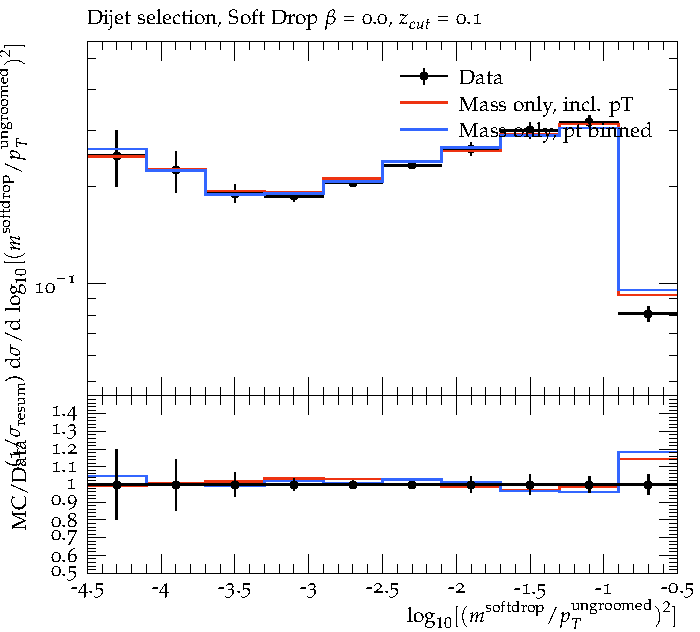
\includegraphics[width=0.49\textwidth]{figs/RivetPlotsMassOnly/SoftDropMass/d01-x01-y01.pdf} \hfill
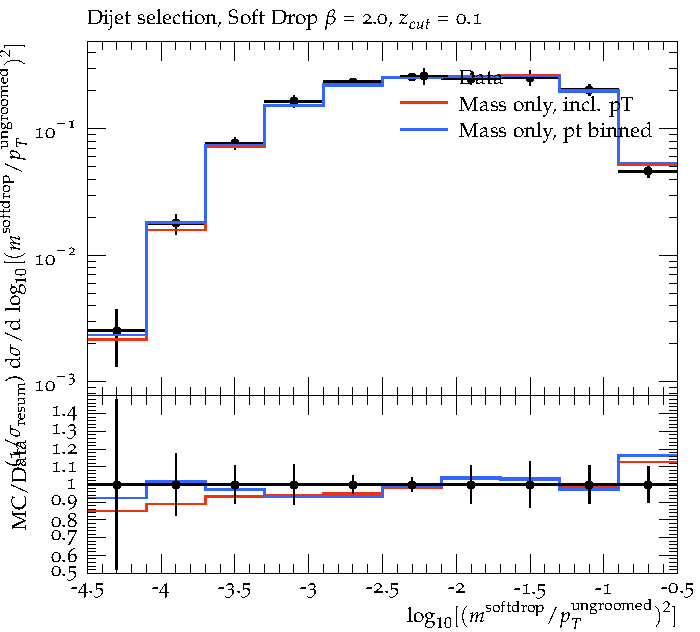
\includegraphics[width=0.49\textwidth]{figs/RivetPlotsMassOnly/SoftDropMass/d03-x01-y01.pdf} \hfill
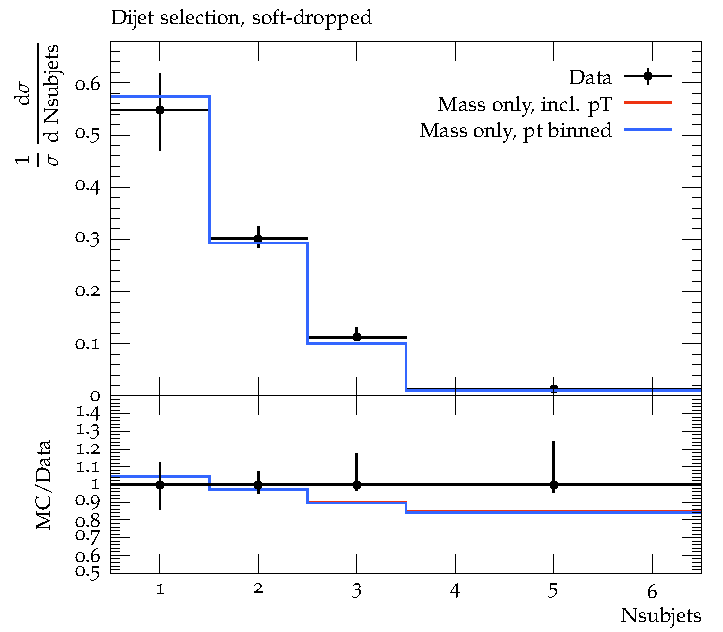
\includegraphics[width=0.49\textwidth]{figs/RivetPlotsMassOnly/ATLAS_2019_I1724098/d23-x01-y01.pdf} \hfill
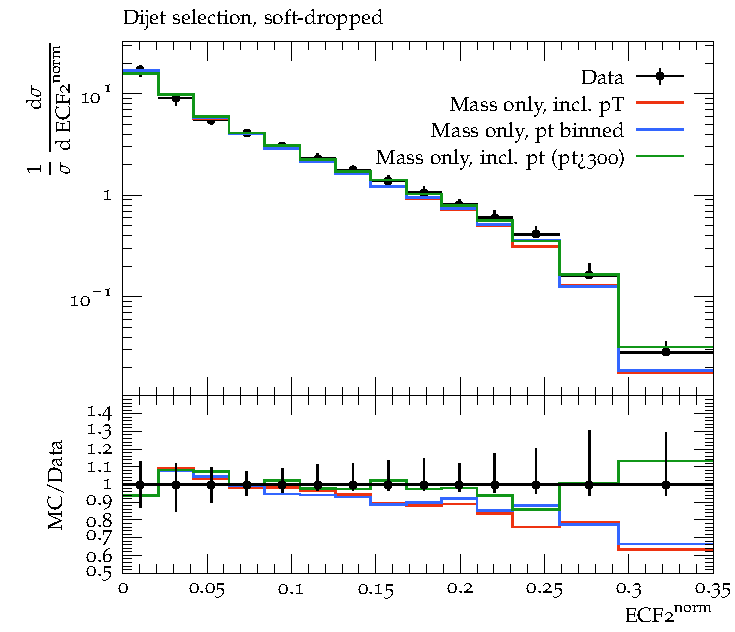
\includegraphics[width=0.49\textwidth]{figs/RivetPlotsMassOnly/ATLAS_2019_I1724098/d27-x01-y01.pdf} \hfill
\end{center}
\label{massOnlyTune}
\end{figure}


The final set of tunes compares the results from each individual measurement. The first of these is the same tune as before, using the $p_T$ inclusive soft drop jet mass measurements at high $p_T$.
The second is the tune using the calorimeter-based measurements of $\rho$, $r_g$, and $z_g$, also inclusive in $p_T$. 
The last tune uses the measurements of several TODO how many jet substructure measurements in jets groomed with the soft drop algorithms, as measured in Ref~\cite{jssObservables}.
These measurements are compared to two standard tunes: the ATLAS A14 tune, and the MONASH tune.
The results of these are shown in Figure~\ref{allTune}. 
A few trends may be seen from these results. In general, the agreement of substructure observables is improved by the use of substructure measurements compared to the ATLAS A14 tune.
As demonstrated in the mass distribution, the tunes from this study seem to lack some information about the fixed-order tune, 
and so they likely need to be combined with other measurements for full accuracy. 
The soft drop jet observables tune is the only tune which accurately reproduces the behavior of $N_{\mathrm{subjets}}$ and $\mathrm{ECF}_2^{\mathrm{norm}}$, though with
degraded agreement for the $\beta=2$ jet mass distribution.


\begin{figure}
\begin{center}
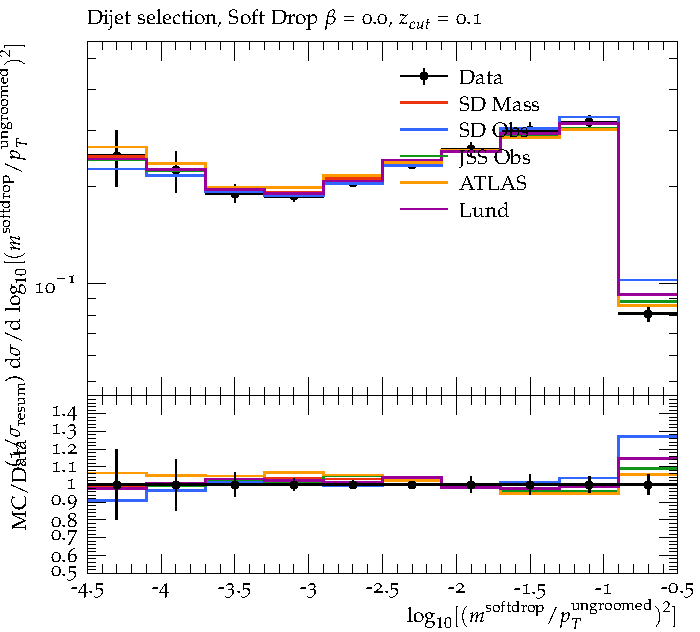
\includegraphics[width=0.49\textwidth]{figs/RivetPlotsFinal/SoftDropMass/d01-x01-y01.pdf} \hfill
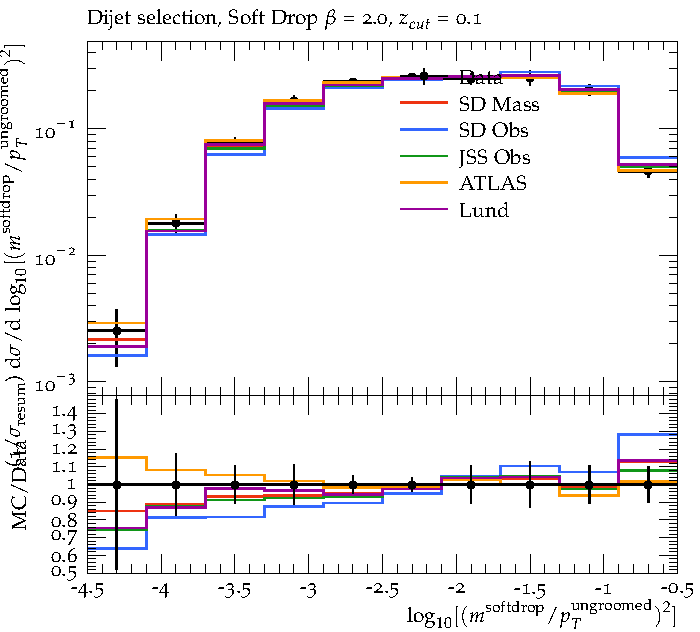
\includegraphics[width=0.49\textwidth]{figs/RivetPlotsFinal/SoftDropMass/d03-x01-y01.pdf} \hfill
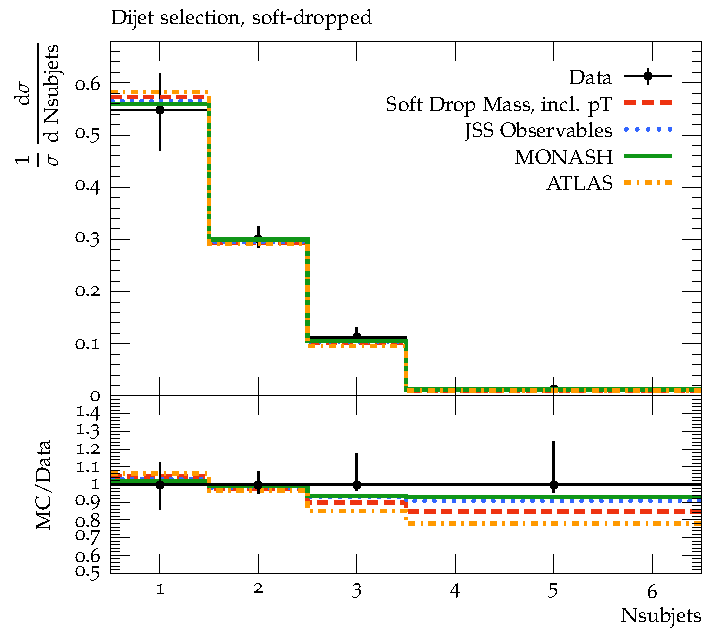
\includegraphics[width=0.49\textwidth]{figs/RivetPlotsFinal/ATLAS_2019_I1724098/d23-x01-y01.pdf} \hfill
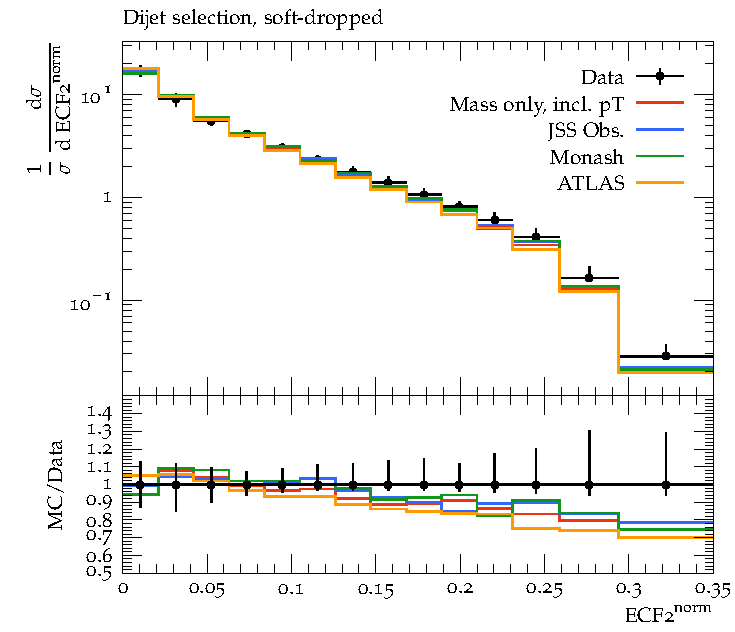
\includegraphics[width=0.49\textwidth]{figs/RivetPlotsFinal/ATLAS_2019_I1724098/d27-x01-y01.pdf} \hfill
\end{center}
\label{allTune}
\end{figure}


The full set of tuned parameters and their uncertainties is shown in Table~\ref{tuneResults}. 
While the agreement of a specific observable typically cannot be linked directly linked to a single tuned parameter, some trends are observed.
Tunes produced from Ref~\cite{softdropObs} tend to have a larger value for TimeShower:alphaSvalue. No other obvious trends can be seen compared to the high-$p_T$ mass tunes, 
indicating that this could be related to the slope seen for the soft drop $\beta=2$ mass distribution.
Tunes produced from Refs~\cite{softdropObs} and ~\cite{jssObs} tend to have higher values of SigmaProcess:alphaSvalue, though both of these measurements are not too sensitive to the hard process.


\clearpage
\begin{landscape}
\begin{table}[ht!]
\caption{Values of tuned parameters.}
\centering\begin{tabular}{ | c | | c | c | c | c | c |} \hline
                                     & MONASH   & ATLAS  & SDM Incl Pt   & SDM Pt Binned & JSS Observables  \\ \hline
SigmaProcess:alphaSvalue             &  0.130   & 0.144  & 0.126+/-0.003 & 0.126+/-0.001 & 0.133+/-0.002 \\ \hline
BeamRemnants:primordialKThard        &  1.8     & 1.72   & 1.825+/-0.055 & 1.794+/-0.011 & 1.785+/-0.048 \\ \hline
SpaceShower:pT0Ref                   &  2.0     & 1.30   & 1.668+/-0.100 & 1.744+/-0.078 & 1.721+/-0.121 \\ \hline
SpaceShower:pTmaxFudge               &          & 0.95   & 1.150+/-0.054 & 1.071+/-0.014 & 1.036+/-0.034 \\ \hline
SpaceShower:pTdampFudge              &          & 1.21   & 1.214+/-0.058 & 1.157+/-0.011 & 1.284+/-0.040 \\ \hline
SpaceShower:alphaSvalue              &  0.1365  & 0.125  & 0.123+/-0.003 & 0.126+/-0.001 & 0.130+/-0.003 \\ \hline
TimeShower:alphaSvalue               &  0.1365  & 0.126  & 0.132+/-0.001 & 0.131+/-0.001 & 0.133+/-0.000 \\ \hline
StringPT:sigma                       &  0.335   &        & 0.348+/-0.003 & 0.350+/-0.003 & 0.333+/-0.006 \\ \hline
MultipartonInteractions:pT0Ref       &  2.28    & 1.98   & 2.000+/-0.100 & 2.181+/-0.049 & 2.441+/-0.148 \\ \hline
MultipartonInteractions:alphaSvalue  &  0.130   & 0118   & 0.116+/-0.003 & 0.126+/-0.002 & 0.128+/-0.003 \\ \hline
\end{tabular}
\label{tab:tuneResults}
\end{table}\end{landscape}
\clearpage



More study is needed in order to fully understand the implications of these results, but there are a few interesting comments. 
The high-$p_T$ soft drop jet mass distribution was designed to study perturbative QCD, but also had several bins sensitive to non-perturbative effects. 
With these preliminary studies, it appears to be as effective in tuning as Ref~\cite{jssObs}, even though it uses fewer observables. 
This is likely due to the factorization of different effects in the soft drop mass distribution, allowing it to be simultaneously sensitive to fixed order effects, the parton shower, and hadronization. 
This shows that factorization is important, and that it is important to be sensitive to a variety of effects when creating these tunes.









Rivet~\cite{Buckley:2010ar}, Professor~\cite{Buckley:2009bj}, HepData~\cite{Buckley:2010jn,Maguire:2017ypu}.  Table with routines (and new ones from this workshop).  See \href{https://twiki.cern.ch/twiki/bin/view/LHCPhysics/LHCJetSubstructureMeasurements}{this twiki}.


\subsection{Probing higher-order effects in PSMC}
\label{sec:jets:psmc}

\subsubsection{Triple Collinear Splitting Functions}
(Ben, Eric, Stefan Prestel)


This study aims at exposing, with the help of energy flow 
networks~\cite{Komiske:2018cqr}, new features of jets induced by higher-order
corrections to parton showers, using the Dire parton shower~\cite{Hoche:2015sya}
as a test case.

Parton shower programs are an an important aspect
of LHC phenomenology, since they imprint perturbative all-order effects onto the
jet structure produced by Event Generators. As such, they serve two primary
purposes: $1)$ the distribution of low-multiplicity
(hard-scattering) states over states of arbitrarily high multiplicity, as well
as $2)$ generating the effect of resummation for observable depending only on 
low-multiplicity configurations. These two goals often lead to conflicting
requirements, as e.g.\ choices to improve
$2)$ often limit the potential to improve $1)$ -- and vice versa. Luckily,
these conflicts are not directly apparent at lowest (i.e.\ leading) order. This
has resulted in parton showers being ``stuck" at leading-order 
(leading-logarithmic) accuracy in their description of emission and 
no-emission rates. With increased demand for more precise event generation, 
improved parton showers will become necessary at the LHC and beyond. For 
example, the use of NLO PDFs (as e.g.\ mandated in NLO+PS
matching) in the parton shower in principle requires parton showers beyond
lowest order.

One way to improve the all-order behavior of the parton shower (point $2)$ 
above) while preserving a systematically improvable state distribution (point $1)$ 
above) is to consistently include higher-order and higher-multiplicity 
splitting functions in the parton 
shower~\cite{Li:2016yez, Hoche:2017iem,Dulat:2018vuy}. Some of the 
necessary ingredients at NLO are shown in 
Fig.~\ref{fig:jets:np:triplecollineardiagrams}. 
At leading order, these configurations are approximated through the iterated 
application of leading-order splittings. This approximation however may
yield an incorrect distribution\footnote{\dots e.g.\ if the polarisation of 
the intermediate gluon in 
Figs.~\ref{fig:jets:np:triplecollineardiagrams1}-\ref{fig:jets:np:triplecollineardiagrams4},
\ref{fig:jets:np:triplecollineardiagrams7}-\ref{fig:jets:np:triplecollineardiagrams8}
is omitted, leading to an incorrect modulation of azimuthal angles,
or by disregarding the interference between
$C_F$-type and $C_A$-type color structures from 
Figs.~\ref{fig:jets:np:triplecollineardiagrams7}-\ref{fig:jets:np:triplecollineardiagrams8}.}
or may be limited to phase-space regions constrained by successive 
ordering requirements\footnote{\dots easily leading to the 
incorrect overall phase space volume, and thus failing to recover known anomalous
dimensions upon integration.}.
The correct final result is obtained by including the 
complete configurations~\ref{fig:jets:np:triplecollineardiagrams}
as new rates in the parton shower, and subtracting from these new rates
the leading-order result. This subtraction will, given a suitable definition
of the leading-order shower, act to ensure local finiteness of the new, 
subtracted, rates. We will call these subtracted rates ``NLO corrections".

In~\cite{Hoche:2017iem}, triple-collinear corrections from diagrams
similar to~\ref{fig:jets:np:triplecollineardiagrams2} were considered, with
the difference that instead of the primary parton (indicated with a double 
line), one of the quarks in the loop was considered as ``hard". Such
configurations give, upon integration, give rise to the flavor-changing 
DGLAP kernels $P_{qq'}$ and $P_{q\bar q}$. We will call this 
``triple-collinear" correction. The calculation of these corrections has
helped define a method to use the overlap with lowest order to construct 
locally finite splitting rates at NLO. Numerically however, this correction is 
expected to be small to modest.
The soft limits of all the diagrams~\ref{fig:jets:np:triplecollineardiagrams}
was considered in~\cite{Dulat:2018vuy}, which also included all necessary 
virtual corrections obtained by moving the cuts in the individual diagrams in 
all possible ways. We will call this ``double-soft" correction\footnote{
It should be noted that there is overlap between the
triple-collinear and double-soft limits. A complete differential calculation 
that consistently (i.e.\ without overlap) includes all components has yet
to be produced. Thus, we assess the potential to find observables
that discriminate between leading-order and next-to-leading order
results separately, for triple-collinear, and for double-soft corrections.}. 
The numerical effect of these double-soft corrections is expected to be appreciable.

In this study, we use the implementation of the triple-collinear and 
double-soft corrections in Dire to produce NLO pseudo-data, with the aim
of highlighting the characteristic new features of either correction.

\vspace*{3ex}
{\bf Maybe now Eric should take over?}
\vspace*{3ex}

Results?:
\begin{itemize}
\item We find that the effect triple-collinear corrections (which integrate to
the DGLAP kernels $P_{qq'}$ and $P_{q\bar q}$) is difficult to pinpoint. 
It is somewhat surprising that the impact is almost vanishing.
\item We find that double-soft corrections have sizable impact, and can
easily be filtered out of the data. This is expected, since the theoretical
description of soft gluons changes significantly.
\end{itemize}

\begin{figure}[h!]
\subfigure[blub]{
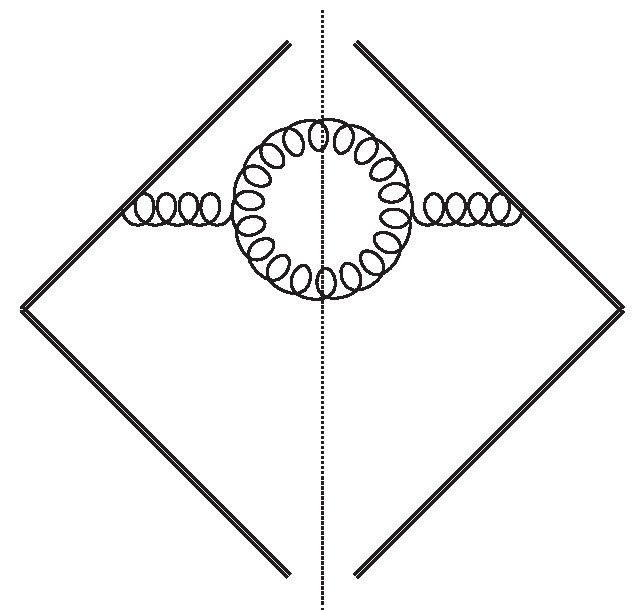
\includegraphics[width=0.23\textwidth]{figs/nlo_real_vpcg.pdf}
\label{fig:jets:np:triplecollineardiagrams1}
}
\subfigure[blub]{
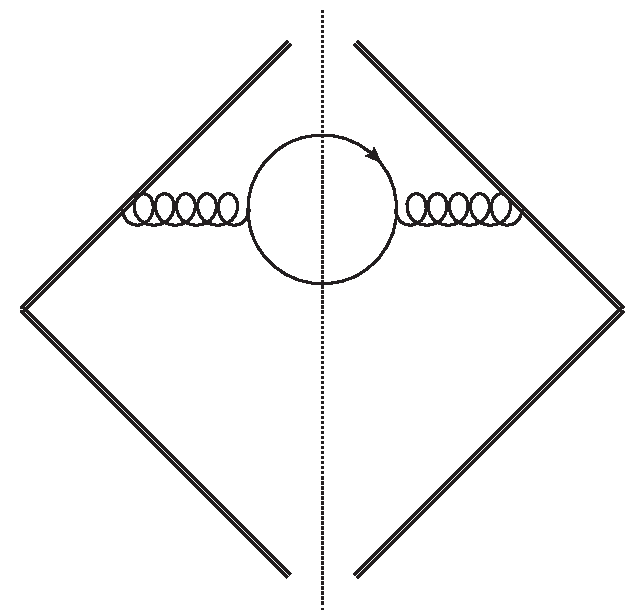
\includegraphics[width=0.23\textwidth]{figs/nlo_real_vpcq.pdf}
\label{fig:jets:np:triplecollineardiagrams2}
}
\subfigure[blub]{
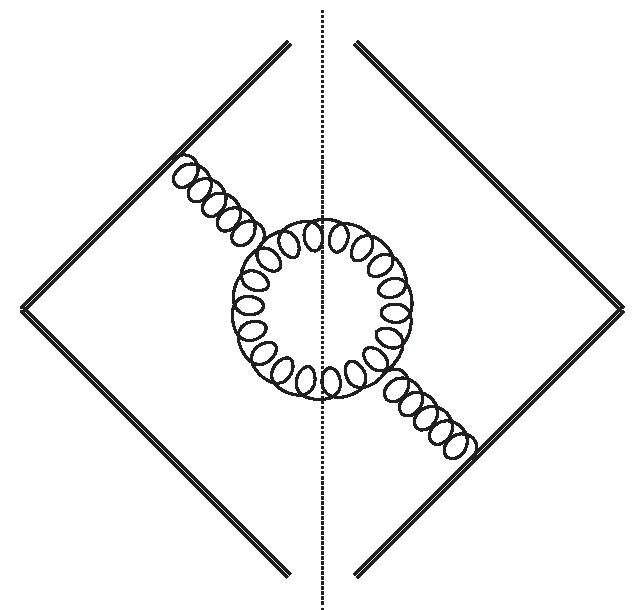
\includegraphics[width=0.23\textwidth]{figs/nlo_real_vpsg.pdf}
\label{fig:jets:np:triplecollineardiagrams3}
}
\subfigure[blub]{
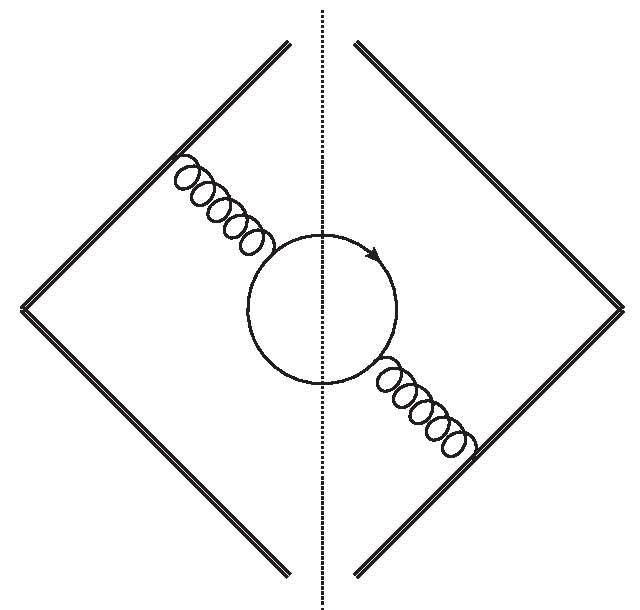
\includegraphics[width=0.23\textwidth]{figs/nlo_real_vpsq.pdf}
\label{fig:jets:np:triplecollineardiagrams4}
}
\\
\subfigure[blub]{
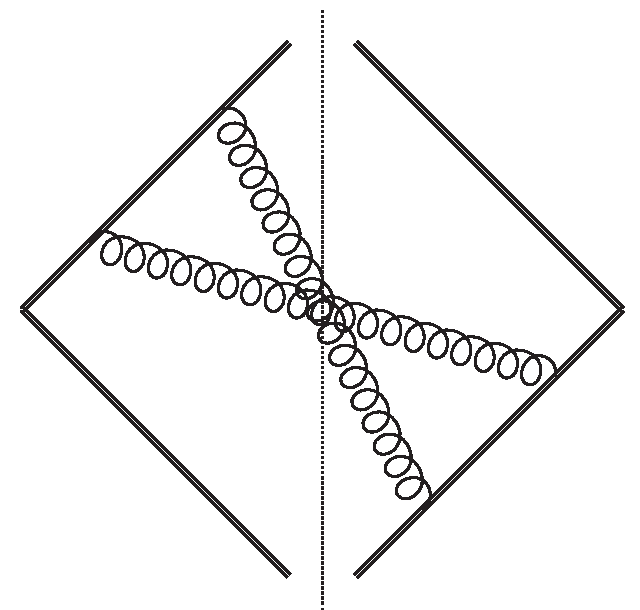
\includegraphics[width=0.23\textwidth]{figs/nlo_real_box1.pdf}
\label{fig:jets:np:triplecollineardiagrams5}
}
\subfigure[blub]{
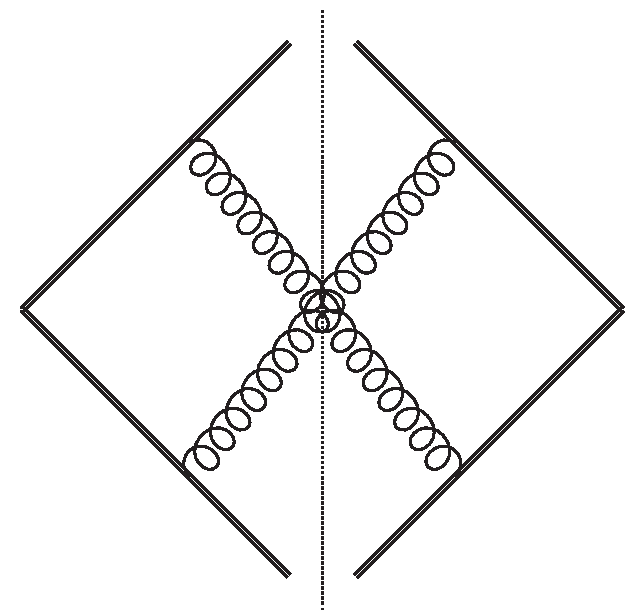
\includegraphics[width=0.23\textwidth]{figs/nlo_real_box2.pdf}
\label{fig:jets:np:triplecollineardiagrams6}
}
\subfigure[blub]{
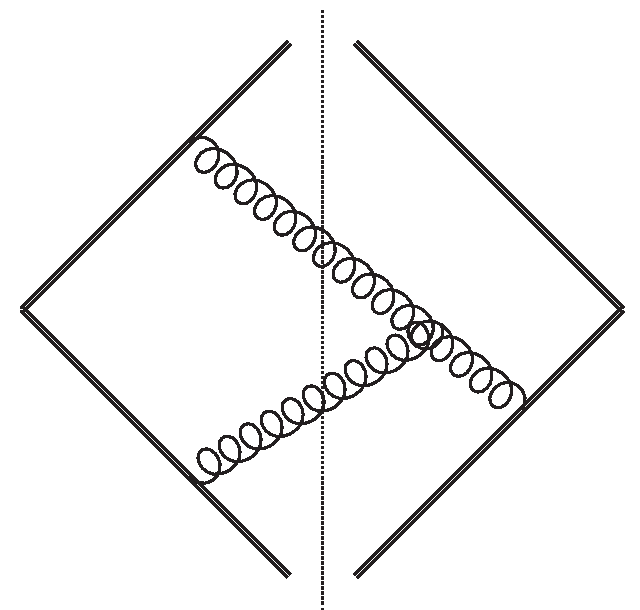
\includegraphics[width=0.23\textwidth]{figs/nlo_real_tgc1.pdf}
\label{fig:jets:np:triplecollineardiagrams7}
}
\subfigure[blub]{
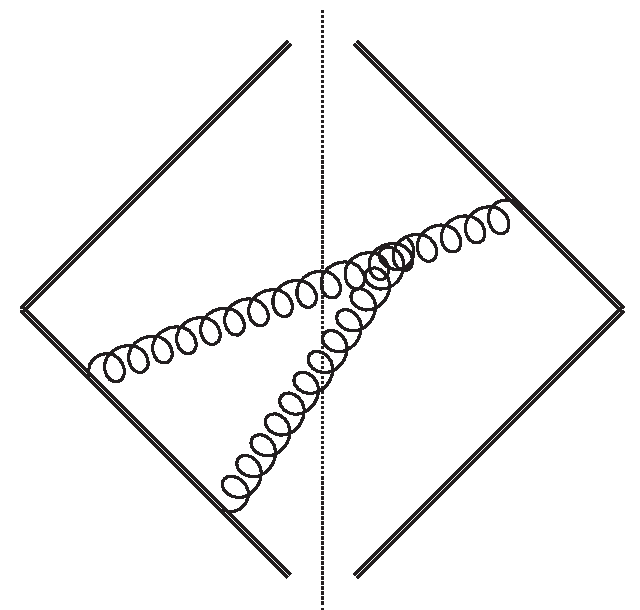
\includegraphics[width=0.23\textwidth]{figs/nlo_real_tgc2.pdf}
\label{fig:jets:np:triplecollineardiagrams8}
}
\caption{Replace me with proper diagrams!}
\label{fig:jets:np:triplecollineardiagrams}
\end{figure}

\begin{figure}[h!]
\centering
\includegraphics[width=0.85\textwidth]{figs/triplecollinear.pdf}
\caption{Replace me with proper plots!}
\label{fig:jets:np:triplecollinearNN}
\end{figure}








\subsection{q/g tagging in VBF and VBS}
\label{sec:jets:vbsbvf}
(Ben, Yachine, Kenneth, Paolo)



\subsection{\textsc{Squirrel} for the Gluon PDF}
\label{sec:jets:pdf}

Parton Distribution Functions (PDFs) describe the non-perturbative dynamics of quarks and gluons in the protons that take part in high-energy collisions. Therefore, they are a key ingredient for every theoretical prediction that aims to describe particle interactions at high-energy colliders such as the LHC. As a consequence, their precise determination is of utmost importance for LHC phenomenology. 
%
The non-perturbative nature of PDFs hampers their determination from first principles.
%
However, for inclusive enough processes, they are universal, i.e.\, up to power corrections, they do not depend on the particular process, and they can be determined by fitting data from previous experiments. Moreover, although they are themselves non-perturbative objects, their dependence on the energy is governed by the DGLAP equation and the evolution kernels can be computed as a power expansion in the strong coupling. This implies that data collected at past experiments, at different energies, can be used to constrain PDFs. 

Traditionally, the main source of uncertainties assigned to the determination of PDFs arises from the experimental error of the data that enter the fit.~\footnote{Very recently, the inclusion of theory uncertainties in PDF determination has also been achieved~\cite{Harland-Lang:2018bxd,AbdulKhalek:2019ihb,AbdulKhalek:2019bux}} In extreme regions of phase-space, for instance at small- or large-$x$, the experimental uncertainties typically deteriorate and one has to face a reduced number of data points. This is reflected in PDFs which are largely unconstrained in these regions. 
%
For instance, the large PDF uncertainty in the $x\to 1$ region, also known as the threshold region, has a negative impact on searches for new and heavy states.
%
 Although this will probably not wash out a potential discovery, it will definitely obscure the nature and the properties of the new state, such as its mass and its couplings. 
%
The way to reduce this PDF uncertainty is to include in the fit data at larger $x$. However, this raises interesting theoretical issues, because fixed-order perturbation theory becomes less reliable as $x$ becomes close to unity and one should supplement theoretical predictions with threshold resummation, as studied for instance in~\cite{Corcella:2005us,Sato:2013wea,Westmark:2013vea,Bonvini:2015ira,Accardi:2014qda}.


In this study, we focus on the gluon PDF in the region of relatively large longitudinal momentum fraction, $x\sim 10^{-1}$. The datasets that mostly constrain the gluon in this region are the inclusive jet spectra, in the region of the jet transverse momentum above 1~TeV and the production of top quark pairs. From a theoretical point of view, both processes are known to very high accuracy, i.e. next-to-next-to-leading order (NNLO)~\cite{Czakon:2015owf,Currie:2016bfm}. Phenomenologically, the two processes have pros and cons. Inclusive jet production features high statistics across a wide kinematical range and, consequently, even in the high $p_t$ region we are interested the experimental uncertainties do not exceed 10\%. However, because one measures inclusive jets, one cannot distinguish the flavour content and the cross section is dominated by quark-quark scattering, which bears little information about the gluon PDF. 
%
On the other hand, at LHC energies, top pair production is dominated by gluon fusion and therefore offers a direct probe of the gluon luminosity. In this case, however, we pay a much higher price in terms of experimental uncertainties, essentially because we run out of statistics for values of the top transverse momentum much smaller than what is reached in the case of inclusive jets. 
%
Ideally, we would like to exploit the vast jet samples collected by the LHC experiments to tease out more information about the gluon PDF. We immediately realise that one way of achieving this scope would be to supplement the inclusive jet $p_t$ spectrum with some information about the jet flavour. 
%
Therefore, in this section, we are going to explore the possibility of using the \emph{inclusive gluon-jet $p_t$} spectrum to extract parton densities, rather than its flavour-blind version. Properly defining quark jets versus gluon jets is a very active area of jet substructure (for a review, see for instance~\cite{Marzani:2019hun}) and indeed it was one of the focus of a past edition of the Les Houches proceedings~\cite{Badger:2016bpw} (see also the follow-up study~\cite{Gras:2017jty}). 


\begin{figure}
\begin{center}
\includegraphics[width=0.49\textwidth, page=9]{figs/fractions.pdf} \hfill
\includegraphics[width=0.49\textwidth, page=10]{figs/fractions.pdf}
\caption{Born-level studies of the flavour composition of dijet events at $\sqrt{s}=13$~TeV, as a function of the jet transverse momentum. The plot on the left shows the fractions of quark-initiated and gluon-initiated processes that contribute to a $gg$ final state. The plot of the right instead shows the fractional composition of the final state for any initial state.}
\label{fig:born_studies} 
\end{center}
\end{figure}

Before discussing how we can sensibly attach a flavour tag to a jet, let us perform a zeroth order test of this idea. Let us assume that we can indeed tag a gluon jet in the final state. Then, the obvious question we should ask ourselves is how strongly the flavour of the final state, which we measure, is correlated with the flavour of the initial state, which intimately related to the parton densities we want to study. 
%
We can easily assess this correlation at Born level by explicitly considering $2 \to 2$ parton scattering and focussing on the two-gluon ($gg$) final state. The left-hand plot of Fig.~\ref{fig:born_studies} shows the fraction of the $gg$ final state that originates from quark-anti-quark initial state ($q \bar q \to gg$) in red and the one from gluon-gluon initial state ($gg \to gg$)  in blue, as a function of the final-state transverse momentum for proton-proton collisions at $\sqrt{s}=13$~TeV (the plot uses the NLO PDF set CT14~\cite{Dulat:2015mca}). 
%
The result of this very first study is rather encouraging: in the region $p_t=1\div2$~TeV we are interested in, there is indeed very strong correlation between the initial- and final-state flavours. This is, of course, only a Born-level study and we can reasonably expect this correlation to deteriorate at higher-orders mostly due to wide-angle radiation. 
%
Although a quantitative estimate of these effects goes beyond the scope of these proceedings, we do not expect them to be dramatic. In any case, one could in principle reduce such contributions with jet grooming. 
%
With the same Born-level setup, we can study how the different partonic final-states contribute to the inclusive cross section. This is shown on the right-hand plot of Fig.~\ref{fig:born_studies}. As $p_t$ increases, the fraction of final-state quark rapidly increases. Indeed, the region of interest the $gg$ final state represents less than 10\% of the inclusive sample. This makes the enterprise of enhancing the $gg$ contributions (or, equivalently, suppressing the quarks) particularly challenging. 



\begin{figure}
\begin{center}
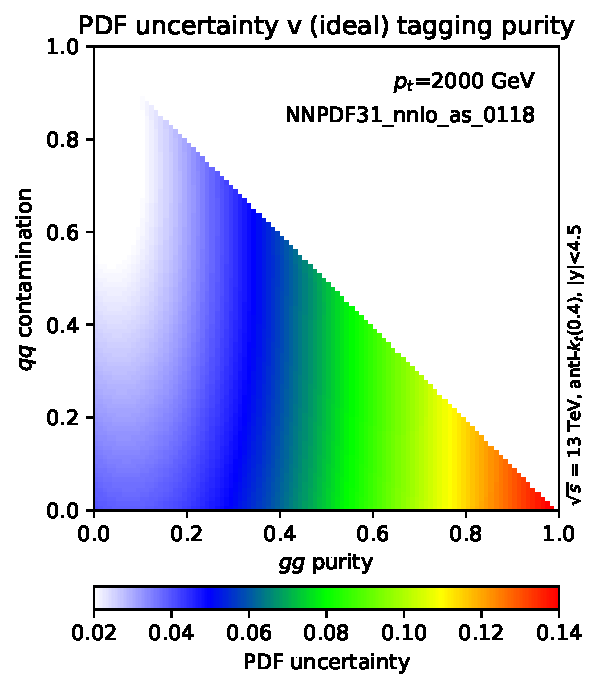
\includegraphics[width=0.42\textwidth, page=1]{figs/performance-plots.pdf} \hfill
\includegraphics[width=0.49\textwidth, page=2]{figs/performance-plots.pdf}
\caption{The plot on the left shows the PDF uncertainty, evaluated using the NNLO set from NNPDF3.1 as a function of $gg$ purity and $qq$ contamination, as defined in the text.
%
The plot on the right shows how the PDF uncertainty compared to experimental systematic and statistical uncertainties, as a function of the $gg$ purity, assuming that  gluon jets have been identified using a tagger with efficiency $\varepsilon_g=0.42$.}
\label{fig:pdf_unc_studies} 
\end{center}
\end{figure}

The next step in our study is to evaluate the current PDF uncertainties, as a function of the final-state flavour composition. 
%
In order to do so, we imagine as a fist step to have at our disposal an idealised tagging procedure that allows us to freely enhance or depress the different partonic components of the final state. We will come back to actual realisations of this tagger later. 
%
In this context, we find useful to define the gluon-gluon ($gg$) purity as
\begin{equation}\label{gg-purity}
gg \, \text{purity}= \frac{\sigma_{gg}}{\sigma_{qq}+\sigma_{qg}+\sigma_{gg}},
\end{equation}
where $\sigma_{ij}$ is the cross section for producing parton $i$ and $j$, evaluated at Born level.  In an analogous way, we can also define the $q q$ contamination, while $q g$ is then fixed by unitarity. 
%
For instance, we already know from Fig.~\ref{fig:born_studies}, that the inclusive, i.e.\ untagged, case correspond to $gg$ purity of the order 5\% at $p_t=2$~TeV, while $qq$ and $qg$ makes up roughly 55\% and 40\% of the inclusive sample, respectively. 

%
The PDF uncertainty on the jet cross section, for given values of $gg$ purity and $qq$ is shown in Fig.~\ref{fig:pdf_unc_studies}, on the left. The plot is obtained using the NNLO PDF set from NNPDF3.1~\cite{Ball:2017nwa} for jets at $2$~TeV.
 %
%The results are shown in Fig.~\ref{fig:pdf_unc_studies}, on the left. 
%
%
From the plot, we see that PDF uncertainty for 5\% $gg$ purity and 55\% $qq$ contamination, which roughly corresponds to the inclusive, i.e.\ untagged, jet cross section at 2~TeV, then is of the order of a few percent.
%
This reflects the fact that the quark parton densities are fairly-well constrained in the region of interest. 
%
As we move to higher values of the $gg$ purity, the less constrained gluon PDF starts to play a more significant role and, as a consequence, the overall uncertainty goes up. For instance, if we were able to devise a tagger that purifies the $gg$ final state to 80\%, we would increase the PDF uncertainty from 2\% to 12\%. 

We can now attempt to assess how good a tagger we should devise in order for the gluon-jet $p_t$ spectrum to be able to constrain the gluon PDF at relatively large $x$. To this purpose, we would like to achieve a situation where the PDF uncertainty is the largest uncertainty, i.e.\ it dominates over the other theoretical and experimental uncertainties. For this feasibility study, we have decided to neglect uncertainties related to the tagging procedure, which can be evaluated, for a given algorithm, using standard scale-variation based, methods. Instead, we concentrate on experimental systematic and statistical uncertainties. These uncertainties are shown on the plot in Fig.~\ref{fig:pdf_unc_studies}, on the right, as function fo the $gg$ purity, for a (yet-to-be-defined) tagging procedure that works at $\varepsilon_g=0.42$ gluon efficiency~\footnote{Instead of fixing the gluon efficiency, we could have specified the $qq$ contamination, which directly corresponds to an horizontal slice of the left-hand plot of Fig.~\ref{fig:pdf_unc_studies}. However, in view of the discussion about taggers that will follow, we find the efficiency more informative.}. 
%
The experimental systematic uncertainty (in dotted red)  is assumed to be a half of the one reported by the LHC collaboration in 2015~\cite{} \sm{Ben can you add the ref please?}, i.e.\ of the order of 5\%. The statistical uncertainty (in dashed green) correspond to an integrated luminosity of 300 fb$^{-1}$, i.e.\ roughly the amount of date collected by the end of Run~III of the LHC.
%
We conclude that the PDF uncertainty becomes the dominant one if the $gg$ purity is above 0.3, for $\varepsilon_g=0.42$. Thus, this sets the goal for our tagger.

\begin{figure}
\begin{center}
\includegraphics[width=0.49\textwidth, page=4]{figs/performance-plots.pdf} \hfill
\includegraphics[width=0.49\textwidth, page=5]{figs/performance-plots.pdf}
\caption{The plot on the left show the tagging performance of the Les Houches energy correlation function and Les Houches multiplicity discussed in this study. 
The ROC curve are obtained using a numerical simulation with the Monte Carlo parton shower Pythia~8.230~\cite{Sjostrand:2014zea}, with the Monash13 tune~\cite{Skands:2014pea} and they are compared to Casimir scaling and the extrapolated performance of a neural-network based tagger that makes use of jet topics~\cite{Metodiev:2018ftz,Komiske:2018vkc}.
The plot on the right show, for each of the tagger (or idealised tagger) we have have considered here, the different sources of uncertainties (namely, PDF, statistical and systematic uncertainties, as a function of the gluon efficiency. 
}
\label{fig:performance_studies} 
\end{center}
\end{figure}
A variety of techniques to define and discriminate quark-initiated versus gluon-initiated jets has been proposed and studied in the literature. It is customary to express a tagger performance in terms of ROC curves, i.e. plots that exhibits the algorithm ability of identify the signal, i.e.\ its efficiency, versus its mis-tag rate. ROC curves for a handful of quark/gluon taggers are shown in Fig.~\ref{fig:performance_studies}, on the left.
%
The plot shows the signal (gluon) efficiency $\varepsilon_g$ on the horizontal axis and the background (quark) efficiency ($\varepsilon_q$) on the vertical axis. The red-line can be take as the reference and it corresponds to so-called Casimir scaling, and it is related to the universal scaling between the colour factor of the fundamental ($C_F$) and adjoint ($C_A$) representations~\cite{Larkoski:2014pca}. 

Because of the different colour factors characterising quark and gluon radiation, gluons tend to radiate more than quarks. Jet shapes such as generalised angularities~\cite{Larkoski:2014pca} and energy-correlation functions (EFCs)~\cite{Larkoski:2013eya} are a probe of such radiation and therefore by selecting jets which exhibit values of the jet shape above a certain threshold, we can enrich our gluon-jet sample. 
% 
Furthermore, jet shapes are fairly-well understood observables and precision-calculations exploiting both fixed-order and resummed perturbation theory are possible, thus systematic reduction of the tagger theoretical uncertainties is, in principle possible. Following the Les Houches studies performed in 2015, the best quark/gluon separation is achieved for the so-called Les Houches ECF, which is characterised by an angular exponent $\alpha=0.5$.
%
The ROC curve for this tagger is shown in green on the left-hand plot of  Fig.~\ref{fig:performance_studies}. We note that despite the fact that jet shapes exhibit Casimir scaling at their lowest order (leading logarithmic accuracy) their discriminating power is increased if higher-order effects are included.
%
The curve has been obtained using a numerical simulation with the Monte Carlo parton shower Pythia~8.230~\cite{Sjostrand:2014zea}, with the Monash13 tune~\cite{Skands:2014pea}.


Given the above consideration, it is natural to wonder if it is possible to find substructure tools
which have a different behaviour already at leading-logarithmic
accuracy.
%
It is well known that counting observables, such as the particle multiplicity in a jet, or the charged-track multiplicity, typically outperform jet shapes as gluon taggers. However, these observables are not infra-red and collinear (IRC) safe. Instead we would like to employ  a counting observable that, unlike the aforementioned multiplicities exhibits IRC safety and therefore can be calculated using perturbation theory. This requirement is particularly important the context we are discussing as one would have to provide a theoretical calculation for a fit of parton densities. 
%
An observable that ticks all these properties is the Iterated SoftDrop (ISD) multiplicity, which was introduced in Ref.~\cite{Frye:2017yrw}.
%
This algorithm applies the SoftDrop procedure~\cite{Larkoski:2014wba} multiple
times, following the hardest branch in
the recursion procedure. This gives a list of
branchings which pass the SoftDrop condition
$(z_1,\theta_1), \dots, (z_n,\theta_n)$. The multiplicity is simply the number of such branchings.
%
It was immediately noticed that for the Iterated SoftDrop multiplicity to IRC safe, one needs either to take a negative value of the SoftDrop angular exponent $\beta$ or impose an explicit cut on the angular separation  $\theta_\text{cut}$.
%
For this study we employ a variant of the SoftDrop iterated multiplicity which is built imposing a minimum relative transverse momentum cut ($k_t=1$~GeV), rather than an angular one. We name this variant of the Iterated SoftDrop multiplicity, the Les Houches multiplicity ($n_\text{LH}$).
The ROC curve for this tagger is shown in blue on the left-hand plot of  Fig.~\ref{fig:performance_studies}. We notice the gain in the performance, while maintaining full calculability. 
%
Finally, the ROC curve shown in black corresponds to an extrapolation of the behaviour obtained with a neural-network (NN) architecture exploiting jet topics~\cite{Metodiev:2018ftz,Komiske:2018vkc}. This idea originates from techniques employed in text-classification and, as the plot shows, outperforms the Les Houches multiplicity at high gluon efficiencies $\varepsilon_g > 0.5$. Measurements of jet topics have already been performed~\cite{Aad:2019onw}, however their theoretical understanding is still in their infancy and whether one can perturbatively predict their behaviour is still work in progress.

For each tagger we want to study, we can now pick an efficiency working point $\varepsilon_g$. Then, the corresponding ROC curve will give us the corresponding miss-tag rate $\varepsilon_q$ and with these two inputs we can estimate a realistic $gg$ purity using Eq.~(\ref{gg-purity});
\begin{equation}\label{gg-purity-after-tagging}
gg \, \text{purity}\Big|_\text{after tagging}= \frac{\sigma_{gg} \varepsilon_g^2}{\sigma_{qq}\varepsilon_q^2+\sigma_{qg}\varepsilon_q \varepsilon_g +\sigma_{gg} \varepsilon_g^2},
\end{equation}
and analogously for $qq$ and $qg$. With this information, we are now ready to compile the final plot of this study, which is shown in Fig.~\ref{fig:performance_studies}, on the right. 
This plot is similar in spirit to the right-hand plot of Fig.~\ref{fig:pdf_unc_studies} but now for actual quark/gluon taggers, rather than an idealised one.
%
As before, we show the different uncertainties: from PDFs ($\delta_\text{PDF}$, solid), statistical uncertainty ($\delta_\text{stat}$, dashed) and systematic one ($\delta_\text{syst}$, dotted). As discussed before, the systematic uncertainty is taken to be constant and equal to 5\%. The statistical uncertainty instead is the square root of the inverse number of the events, and so it  depends on $\varepsilon_g$ (and $\varepsilon_q$). For this, an integrated luminosity of 300~fb$^{-1}$ is assumed. Finally,  the PDF uncertainty of jet cross-section for $p_t>2$~TeV, after tagging is evaluated with NNPDF3.1, as a function of the tagger efficiency. 
%
The plot shows the different uncertainties $\delta_i$ for the taggers mentioned before: a tagger exhibiting simple Casimir scaling (red curves), the Les Houches ECFs (green curves), the Les Houches multiplicity (blue curves) and the neural-network tagger (black curves). The systematic uncertainty is assumed to be the same for each tagger. 
%
The plot shows that for jets with transverse momentum above 2~TeV a pure Casimir-scaling tagger or a ECF-based tagger are never good enough to enrich the final-state gluon content such that $\delta_\text{PDF}> \delta_\text{syst}, \delta_{stat}$.
%
Instead, if we pick $\epsilon_g\simeq 0.5$ the $n_\text{LH}$ tagger and the NN one do provide $\delta_\text{PDF}$ which are comparable, if not definitely bigger, then statistical and systematic uncertainties. This is definitely more marked for the NN tagger but, as mentioned before, it is currently unclear how to perform perturbative calculations for this. On the other hand, the jet transverse momentum distribution with a cut on $n_\text{LH}$ is well-defined and calculable in perturbation theory. 
%
However, in order to reach firmer conclusions of about the ability of these taggers to effectively discriminate between quark-like and gluon-like jets, we would have to add to this study an assessment of the tagging uncertainties. In a Monte Carlo study, this can be estimated by looking at ROC curves obtained with different Monte Carlo event generators, while in the case of an analytic study one can vary the perturbative scales. We leave such studies for future work. 
dis

\subsection{The highest energy gluons at the LHC}
\label{sec:jets:highest}
(Ben)


\subsection{Conclusion and Outlook}
\label{sec:jets:conclusion}
The jet subgroup at Les Houches 2019 concentrated their effort on the study of gluonic jets across four decades of energy, which are explored by the LHC. 
%
In the low-energy regime jets are sensitive to the non-perturbative dynamics of QCD and their description is beyond the jurisdiction of the standard first-principle approach based on perturbative field theory. Therefore, phenomenological models are usually employed to describe the non-perturbative parton-to-hadron transition. 
%
In our study, we have first addressed some of qualitative features of the groomed jet mass distribution in the non-perturbative regime and then turned our attention to the possibility of employing jet substructure variables to test and, eventually, improve on, the modelling of non-perturbative corrections in Monte Carlo event generators. 

As we go up in energy, we enter the regime where we expect parton-shower algorithms to correctly capture the relevant physics. In this context, we have investigated the impact of higher-order corrections to the splitting kernels that are at the core of any parton-branching algorithm. In particular, we have exploited modern machine-learning techniques in order to design observables that are sensitive to triple-collinear and double-soft corrections. 
%
At high energy, the issue of determining whether a given jet can be labelled as quark-initiated or gluon-initiated becomes central in Higgs physics and in the context of searches for particles and interactions beyond the Standard Model. Therefore, we have studied the performance of quark/gluon tagging in vector-boson-fusion and vector-boson-scattering analyses. Inspired by quark/gluon tagging in searches, we have explored the possibility of measuring gluon-jet transverse momentum distributions as a probe of parton distribution functions at high, i.e.\ 1~TeV, scale.
%
Finally, we have discussed how to probe the most energetic gluons at the LHC.


This report testifies that the jet subgroup have enjoyed a fruitful workshop, characterised by lively discussions and cross-pollination of ideas not only between theory and experimental communities but also between different methodologies, such as first-principle calculations in field theory, Monte Carlo simulations and machine-learning techniques. 
%
We are confident that these results, in some cases still preliminary, are already seeding new ideas and research projects which we look forward to further developing at the next edition of this workshop. 	



\subsection*{Acknowledgments}

We thank the participants of Les Houches 2019 for a lively environment and useful discussions.
%%
BN is supported in part by the Office of High Energy Physics of the U.S. Department of Energy under Contract No. DE-AC02-05CH11231.
%
SM is also supported by the curiosity-driven grant ``Using jets to challenge the Standard Model of particle physics" from Universit\`a di Genova.

\bibliography{lh2019}

\end{document}
